\section{Consitution du dossier}

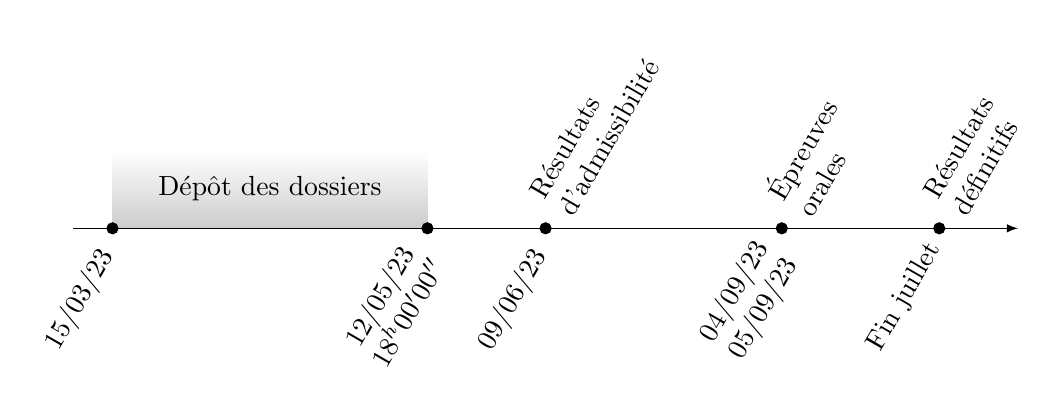
\begin{tikzpicture}
\shade[top color=white, bottom color=black!20!white] (0,0) rectangle (4,1);
\draw[->,>=latex] (-0.5,0)--(11.5,0);
\draw (2,0.5) node{Dépôt des dossiers};
\draw[fill=black] (0,0) circle(.07)node[below=.2cm, rotate=60, anchor=east]{15/03/23};
\draw[fill=black] (4,0) circle(.07)node[below=.2cm, rotate=60, anchor=east, align=center]{12/05/23\\ $18^h\uline{00'00''}$};
\draw[fill=black] (5.5,0)circle(0.07)node[below=.2cm, rotate=60, anchor=east]{09/06/23};
\draw[fill=black] (8.5,0) circle (0.07) node[below=0.2cm, rotate=60, anchor=east, align=left]{04/09/23\\ 05/09/23};
\draw[fill=black] (10.5,0) circle (0.07) node[below=0.1cm, rotate=60, anchor=east]{Fin juillet};

\draw (5.5,0)node[above=.2cm, rotate=60, anchor=west, align=left]{Résultats\\ d'admissibilité};
\draw (8.5,0)node[above=.2cm, rotate=60, anchor=west, align=left]{\'Epreuves\\ orales};
\draw (10.5,0)node[above=.2cm, rotate=60, anchor=west, align=left]{R\'esultats\\ d\'efinitifs};
\end{tikzpicture}

Avant de parler des oraux, il faut tout d’abord te présenter la première phase du concours : l’étude des dossiers. Les dossiers d’admissibilité sont composés de quatre parties majeures :

\begin{enumerate}[label=\arabic*.]
\item \uline{\textbf{La lettre de motivation :}}\\ 
C’est elle qui est la clé de votre admissibilité. Il faut y mettre en valeur votre volonté, vos raisons pour la candidature, vos qualités et les possibilités que le programme vous offrira, en insistant sur les raisons pour lesquelles votre profil correspond au programme.
\item \uline{\textbf{Tes résultats académiques}} (du Bac à la deuxième année de médecine ou de pharmacie) :\\
Il s’agit de vérifier ta capacité de travail, déjà mise en lumière par ta réussite du PASS/L.AS.
\item \uline{\textbf{Les lettres de recommandation :}}\\
Il s’agit d’un pilier de ta candidature. Il importe plus d’avoir des lettres personnalisées de figures compétentes et qui te connaissent \textit{(ex. profs de lycée)} que d’avoir beaucoup de lettres, qui peuvent être parfois impersonnelles.
\item \uline{\textbf{Ton \href{https://drive.google.com/file/d/1cVb_Z6DrBkKD3Q_1rMXHFVpm5KtDrTch/view?usp=sharing}{\textit{Curriculum Vit\ae}}}} qui permet de mettre en valeur tes activités extra-scolaires et professionnelles comme des stages que tu aurais déjà effectués.
\end{enumerate}

\bigskip

Par ailleurs, pour t'aider dans la préparation de ton dossier, \href{https://www.facebook.com/AMPSasso/?locale=fr_FR}{l’AMPS (Association des étudiants en médecine ou pharmacie dans un double cursus)}\footnote{https://www.facebook.com/AMPSasso/?locale=fr_FR} devrait normalement proposer un tutorat pour les dossiers.